\documentclass[red]{beamer}
\usepackage[]{graphicx}\usepackage[]{color}
\usepackage{tcolorbox}
%% maxwidth is the original width if it is less than linewidth
%% otherwise use linewidth (to make sure the graphics do not exceed the margin)
\makeatletter
\def\maxwidth{ %
  \ifdim\Gin@nat@width>\linewidth
    \linewidth
  \else
    \Gin@nat@width
  \fi
}
\makeatother

\definecolor{fgcolor}{rgb}{0.345, 0.345, 0.345}
\newcommand{\hlnum}[1]{\textcolor[rgb]{0.686,0.059,0.569}{#1}}%
\newcommand{\hlstr}[1]{\textcolor[rgb]{0.192,0.494,0.8}{#1}}%
\newcommand{\hlcom}[1]{\textcolor[rgb]{0.678,0.584,0.686}{\textit{#1}}}%
\newcommand{\hlopt}[1]{\textcolor[rgb]{0,0,0}{#1}}%
\newcommand{\hlstd}[1]{\textcolor[rgb]{0.345,0.345,0.345}{#1}}%
\newcommand{\hlkwa}[1]{\textcolor[rgb]{0.161,0.373,0.58}{\textbf{#1}}}%
\newcommand{\hlkwb}[1]{\textcolor[rgb]{0.69,0.353,0.396}{#1}}%
\newcommand{\hlkwc}[1]{\textcolor[rgb]{0.333,0.667,0.333}{#1}}%
\newcommand{\hlkwd}[1]{\textcolor[rgb]{0.737,0.353,0.396}{\textbf{#1}}}%
\let\hlipl\hlkwb

\usepackage{framed}
\makeatletter
\newenvironment{kframe}{%
 \def\at@end@of@kframe{}%
 \ifinner\ifhmode%
  \def\at@end@of@kframe{\end{minipage}}%
  \begin{minipage}{\columnwidth}%
 \fi\fi%
 \def\FrameCommand##1{\hskip\@totalleftmargin \hskip-\fboxsep
 \colorbox{shadecolor}{##1}\hskip-\fboxsep
     % There is no \\@totalrightmargin, so:
     \hskip-\linewidth \hskip-\@totalleftmargin \hskip\columnwidth}%
 \MakeFramed {\advance\hsize-\width
   \@totalleftmargin\z@ \linewidth\hsize
   \@setminipage}}%
 {\par\unskip\endMakeFramed%
 \at@end@of@kframe}
\makeatother

\definecolor{shadecolor}{rgb}{.97, .97, .97}
\definecolor{messagecolor}{rgb}{0, 0, 0}
\definecolor{warningcolor}{rgb}{1, 0, 1}
\definecolor{errorcolor}{rgb}{1, 0, 0}
\newenvironment{knitrout}{}{} % an empty environment to be redefined in TeX

\usepackage{alltt}
\usetheme{Madrid}
\usepackage{graphicx}
\usepackage{xcolor}
\usepackage{media9}

\setbeamertemplate{navigation symbols}{}
\setbeamertemplate{footline}[pagenumber]
\setbeamertemplate{footline}{}


\definecolor{darkpastelgreen}{rgb}{0.01, 0.75, 0.24}
\definecolor{darkorange}{rgb}{1.0, 0.55, 0.0}
\newcommand{\bl}[1]{\textcolor{blue}{#1}}
\newcommand{\rd}[1]{\textcolor{red}{#1}}
\newcommand{\mg}[1]{\textcolor{magenta}{#1}}
\newcommand{\gn}[1]{\textcolor{darkpastelgreen}{#1}}
\newcommand{\org}[1]{\textcolor{darkorange}{#1}}
\setbeamersize{text margin left=15pt,text margin right=25pt}
\usepackage{etoolbox} 
\makeatletter
\preto{\@verbatim}{\topsep=0pt \partopsep=0pt }
\makeatother
\renewenvironment{knitrout}{\setlength{\topsep}{1mm}}{}

\title{Large Data Computation in Python}

% A subtitle is optional and this may be deleted
%\subtitle{Optional Subtitle}

\author{Yujia Deng and Annie Qu}
\institute[UIUC] % Your institution as it will appear on the bottom of every slide, may be shorthand to save space
{
University of Illinois at Urbana-Champaign}
\date{}
\IfFileExists{upquote.sty}{\usepackage{upquote}}{}
\begin{document}

\begin{frame}
  \titlepage
\end{frame}

\begin{frame}
\centering
\LARGE \textcolor{blue}{\textbf{Out-of-memory Data: Pandas+SQL}}
\end{frame}

\begin{frame}
\frametitle{Out-of-memory Data: Pandas+SQL}
\begin{itemize}
	\item NYC's 311 complaints since 2010 (Updated daily): https://data.cityofnewyork.us/Social-Services/311-Service-Requests-from-2010-to-Present/erm2-nwe9
	
	
	\item About \textcolor{blue}{10GB}, \textcolor{blue}{19.6M} records, \textcolor{blue}{41} columns
\end{itemize}
\vspace{-5mm}
\begin{figure}
	\centering
	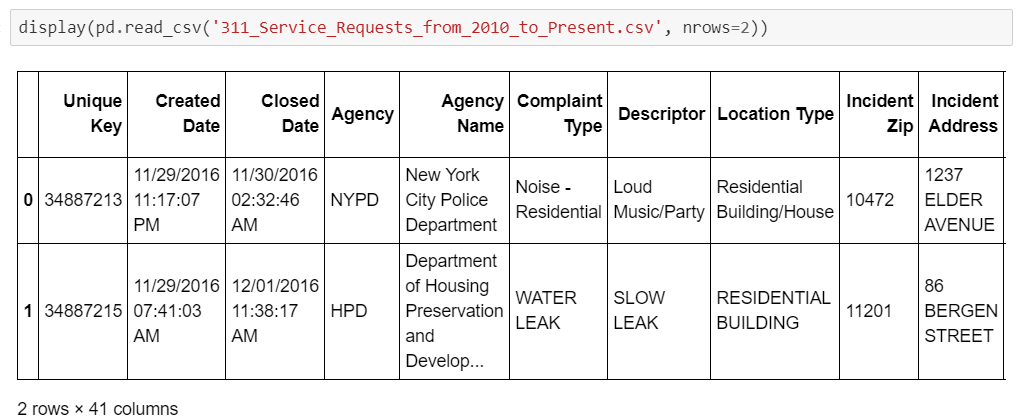
\includegraphics[width=1\linewidth]{figure/screenshot001}
\end{figure}
\end{frame}

\begin{frame}
\begin{itemize}
	\item \textcolor{red}{\texttt{MemoryError}} if we load the whole data at once
	\begin{figure}
		\centering
		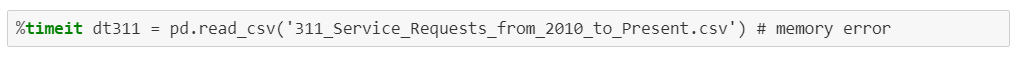
\includegraphics[width=1\linewidth]{figure/screenshot002}
	\end{figure}

	\vspace{3mm}
	\item Create a database and connect using SQL
	\begin{figure}
		\centering
		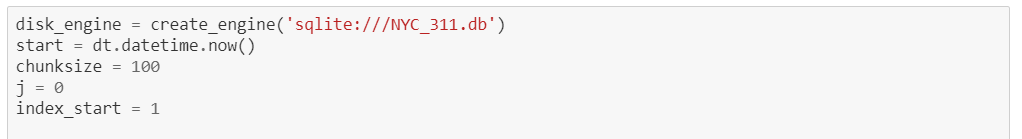
\includegraphics[width=1\linewidth]{figure/screenshot003}
	\end{figure}
\end{itemize}
\end{frame}

\begin{frame}
\frametitle{Read by crunk and subset}
\begin{itemize}
	
	\item Subset and append to the database \textcolor{blue}{chunk by chunk}
	\begin{figure}
		\centering
		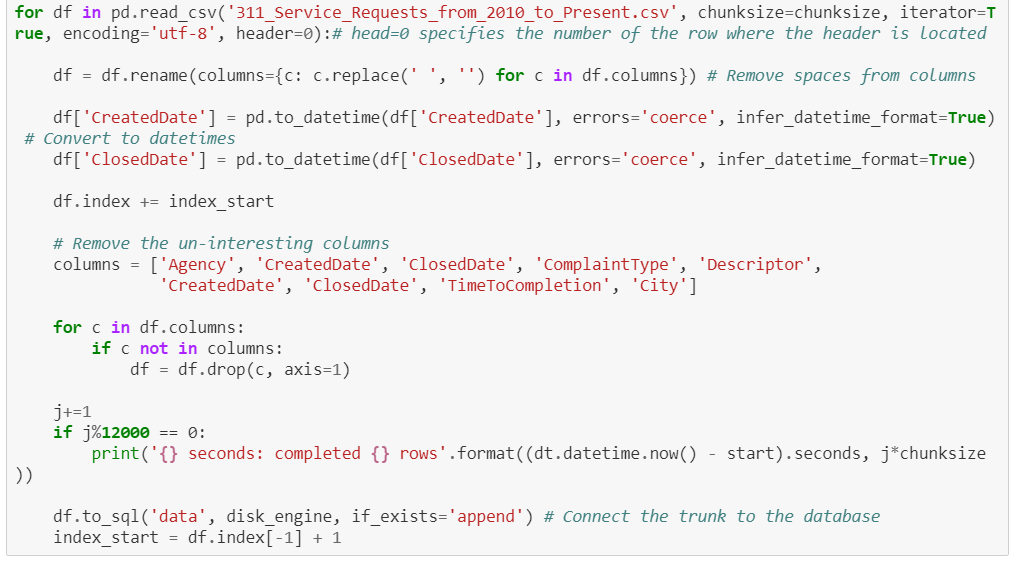
\includegraphics[width=1\linewidth]{figure/screenshot004}
	\end{figure}
	\item Even so, the reading procedure takes more than \textcolor{blue}{4 hours} to complete.
\end{itemize}
\end{frame}

\begin{frame}
\frametitle{Use SQL to explore the data}
\begin{itemize}
	\item Check the total number of records
	\begin{figure}
		\centering
		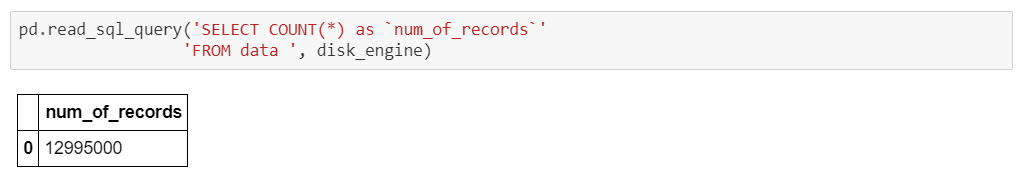
\includegraphics[width=1\linewidth]{figure/screenshot005}
	\end{figure}
\vspace{2mm}
	\item Investigate which department receives the most complaints
	\begin{figure}
		\centering
		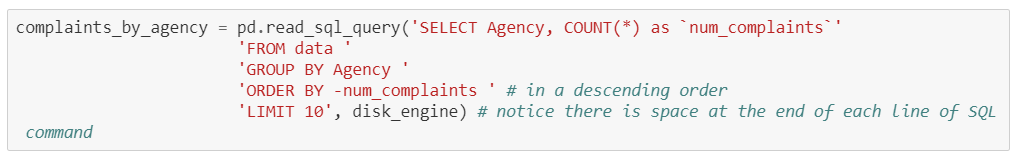
\includegraphics[width=1\linewidth]{figure/screenshot006}
	\end{figure}	
\end{itemize}
\end{frame}

\begin{frame}
\frametitle{Visualization using \texttt{matplotlib}}
\begin{figure}
	\centering
	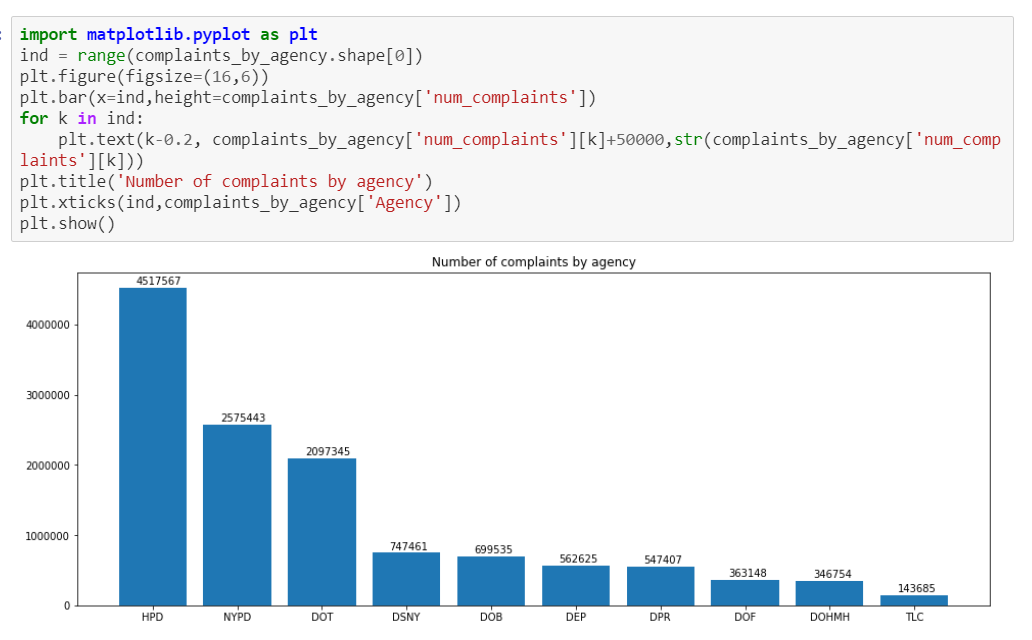
\includegraphics[width=1\linewidth]{figure/screenshot007}
\end{figure}
\vspace{-5mm}
Department of Housing Preservation and Development (HPD) 
\end{frame}

\begin{frame}
\frametitle{Most common complaints}
\begin{itemize}
	\item Similarly, we can investigate what are the most common complaints
	\begin{figure}
		\centering
		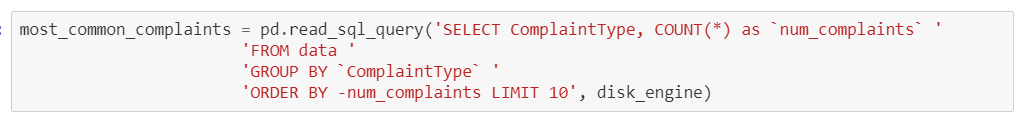
\includegraphics[width=1\linewidth]{figure/screenshot008}
	\end{figure}
	
	\begin{figure}
		\centering
		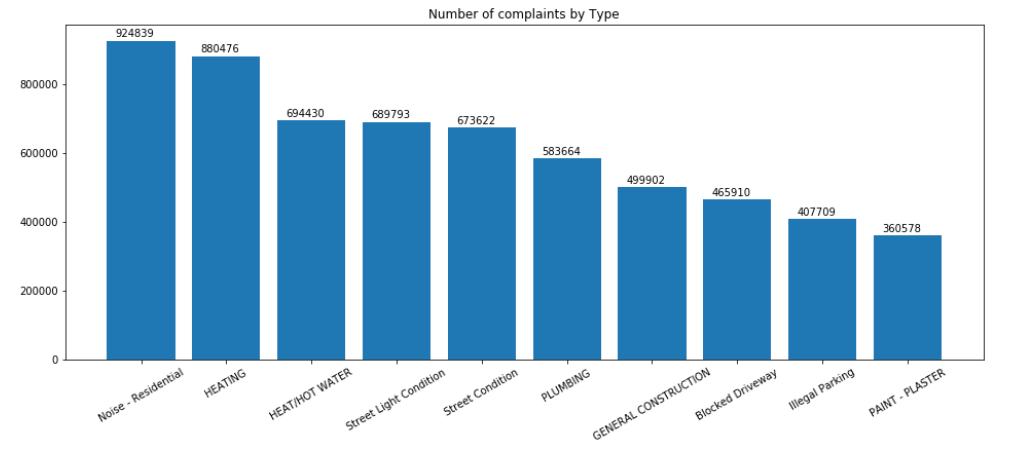
\includegraphics[width=1\linewidth]{figure/screenshot009}
	\end{figure}	
\end{itemize}
\end{frame}

\begin{frame}
\centering
\LARGE \textcolor{blue}{\textbf{Within-memory Data: How to save space}}
\end{frame}

\begin{frame}
\frametitle{Save the memory by specifying the datatype}
\begin{itemize}
	\item Airline data: \textcolor{blue}{3GB}, \textcolor{blue}{7009728} observations, \textcolor{blue}{29} columns
	\item Overview of the datatype
	\begin{figure}
		\centering
		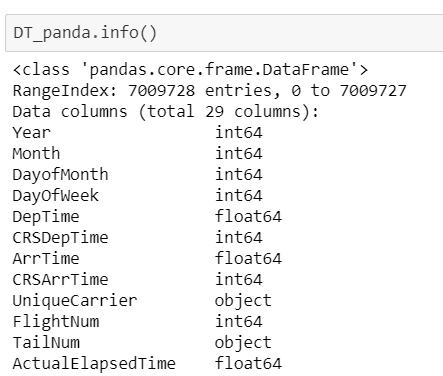
\includegraphics[width=0.6\linewidth]{figure/screenshot010}
	\end{figure}
\end{itemize}
\end{frame}

\begin{frame}
\frametitle{Compress the numerical data}
	\begin{itemize}
		\item \texttt{int64}: ($-2^{64}$ to $2^{64}-1$) and uses \textcolor{red}{8} bytes
		\vspace{2mm}
		
		\item \texttt{int16}:  ($-2^{16}$ to $2^{16}-1$) or (-32,768 to +32,767) and uses only \textcolor{red}{2} bytes. 
		
		\vspace{2mm}
		\item \texttt{pd.to\_numeric(, downcast=)} determines the smallest possible type \textcolor{blue}{automatically}
		\begin{figure}
			\centering
			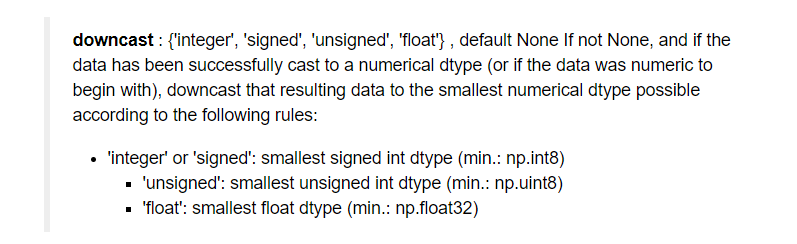
\includegraphics[width=1\linewidth]{figure/screenshot011}
		\end{figure}
		
	\end{itemize}
\end{frame}

\begin{frame}
\frametitle{\texttt{int64} to \texttt{unsigned}}
\begin{itemize}
	\item Check data size change
	\begin{figure}
		\centering
		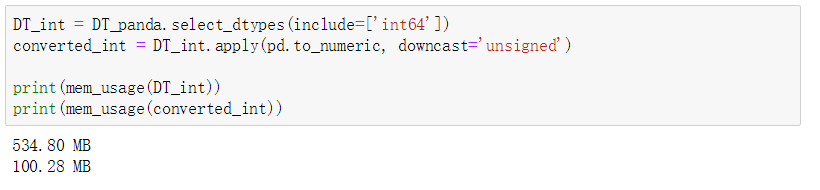
\includegraphics[width=1\linewidth]{figure/screenshot012}
	\end{figure}
	\item Before vs After
	\begin{figure}
		\centering
		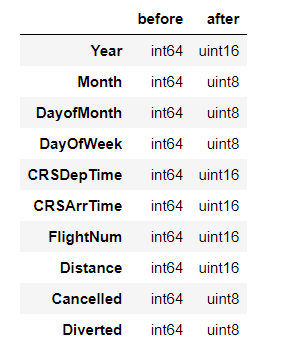
\includegraphics[width=0.4\linewidth]{figure/screenshot013}
	\end{figure}
	
\end{itemize}


\end{frame}

\begin{frame}
\frametitle{\texttt{float} to \texttt{float}}
\begin{itemize}
	\item For \texttt{float} type
	\begin{figure}
		\centering
		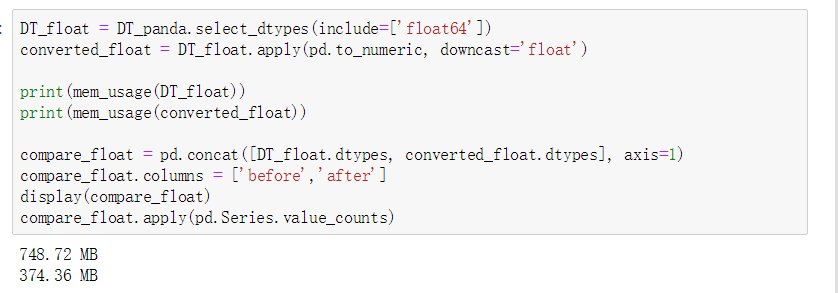
\includegraphics[width=1\linewidth]{figure/screenshot014}
	\end{figure}
	\vspace{-5mm}
	\begin{figure}
		\centering
		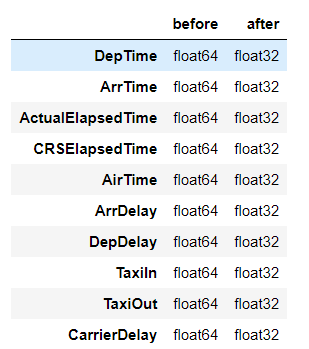
\includegraphics[width=0.4\linewidth]{figure/screenshot015}
	\end{figure}
\end{itemize}
\end{frame}

\begin{frame}
\frametitle{\texttt{object} to \texttt{category}}
\begin{itemize}
	\item \texttt{object} : save strings 
	\begin{figure}
		\centering
		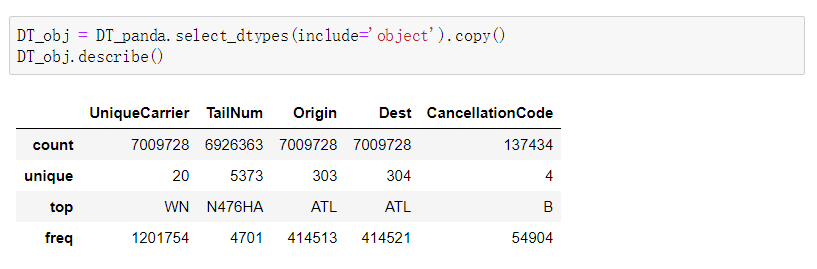
\includegraphics[width=1\linewidth]{figure/screenshot016}
	\end{figure}
	\item \texttt{category} type codes the string into category numbers (similar as factor type in R)
		\begin{itemize}
			\item From: \texttt{array([nan, 'A', 'C', 'B', 'D'], dtype=object)}
			\item To: \texttt{array([-1,  0,  1,  2,  3], dtype=int8)}
		\end{itemize}
	
	\end{itemize}
\end{frame}

\begin{frame}
\frametitle{\texttt{object} to \texttt{category}}
\begin{itemize}
	\item Not economic if there are too many unique values
	\vspace{2mm}
	\item Check if unique value $<$ 50\%
	\begin{figure}
		\centering
		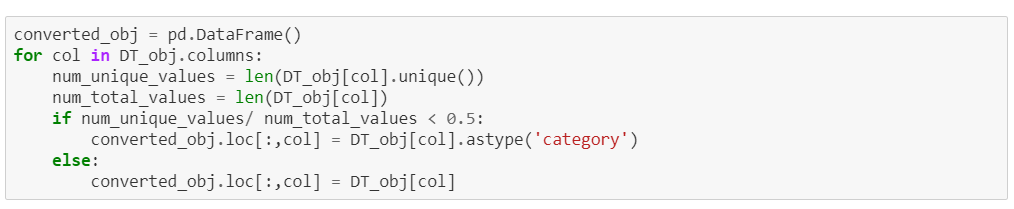
\includegraphics[width=1\linewidth]{figure/screenshot018}
	\end{figure}
	\item Memory saving
	\begin{figure}
		\centering
		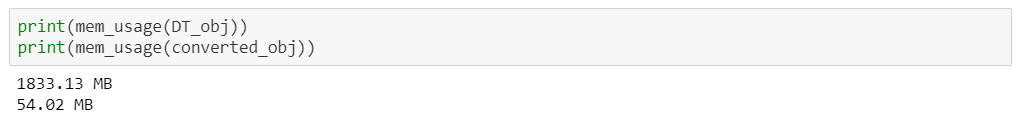
\includegraphics[width=1\linewidth]{figure/screenshot019}
	\end{figure}
\end{itemize}

\end{frame}

\begin{frame}
\frametitle{Prespecify the datatype before loading}
\begin{itemize}
	\item Define the datatype
	\begin{figure}
		\centering
		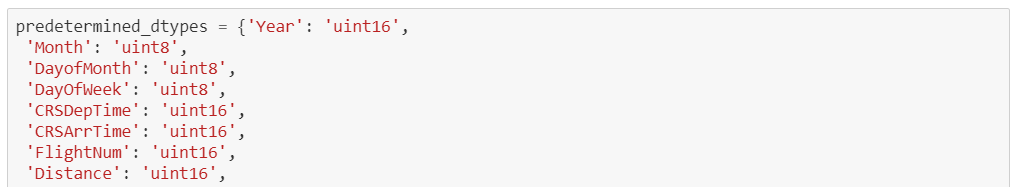
\includegraphics[width=1\linewidth]{figure/screenshot021}
	\end{figure}
	\vspace{-2mm}
	... ...
	\vspace{3mm}
	
\includegraphics[width=1\linewidth]{figure/screenshot022}
	\vspace{3mm}
	\item 528.65 MB vs 3116.65 MB, 83\% saved!
\end{itemize}
\end{frame}


\section{Parallel Computing}
\begin{frame}
\centering
\LARGE \textcolor{blue}{\textbf{Parallel Computing using \texttt{joblib}}}
\end{frame}

\begin{frame}
\frametitle{\texttt{joblib}}
\begin{itemize}
	\item \textcolor{blue}{\texttt{joblib}} is based on \textcolor{blue}{\texttt{multiprocess} }but provides more powerful and flexible methods.
	\item Basic syntax
	\begin{figure}
		\centering
		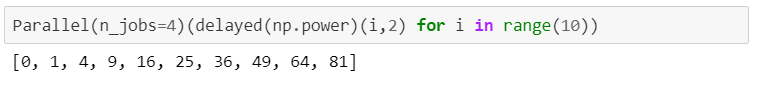
\includegraphics[width=1\linewidth]{figure/screenshot023}
	\end{figure}
	\item Compared with
	\begin{figure}
		\centering
		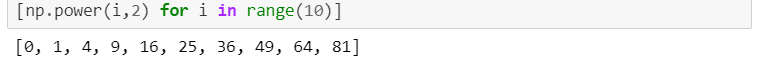
\includegraphics[width=1\linewidth]{figure/screenshot024}
	\end{figure}	
	\item Multiple inputs and multiple outputs
	\begin{figure}
		\centering
		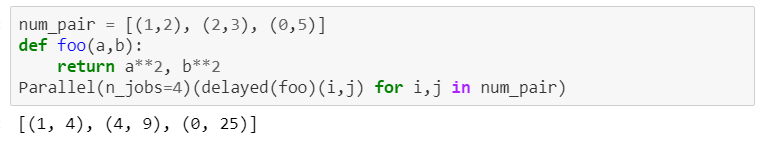
\includegraphics[width=1\linewidth]{figure/screenshot025}
	\end{figure}
\end{itemize}
\end{frame}

\begin{frame}
\frametitle{Example: bootstrap on Iris data}
\begin{itemize}
	\item We use Python to repeat the bootstrap sample on Iris data
	\item Module \textcolor{blue}{\texttt{sklearn}} contains many machine learning methods and commonly used dataset
	\item Load the data from \texttt{sklearn} module
	\begin{figure}
		\centering
		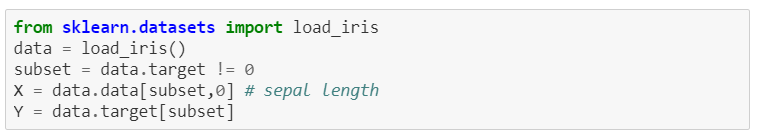
\includegraphics[width=1\linewidth]{figure/screenshot026}
	\end{figure}
	\item Run glm from \texttt{sklearn}
	\begin{figure}
		\centering
		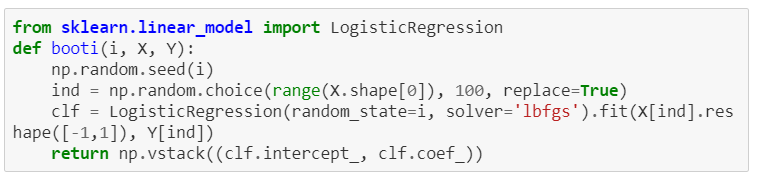
\includegraphics[width=1\linewidth]{figure/screenshot027}
	\end{figure}
\end{itemize}
\end{frame}

\begin{frame}
\frametitle{Example: bootstrap on Iris data}
\begin{itemize}
	\item Sequential way 
	\vspace{-1mm}
	\begin{figure}
		\centering
		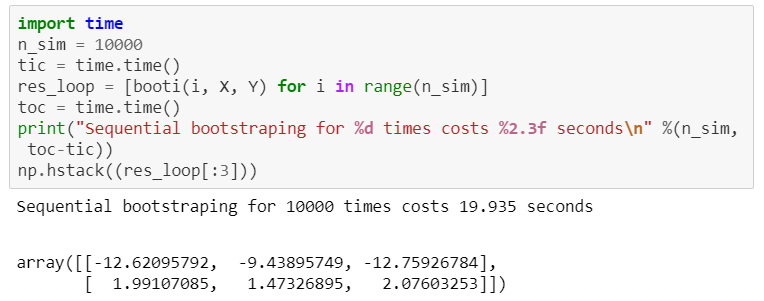
\includegraphics[width=0.85\linewidth]{figure/screenshot028}
	\end{figure}
	
	\vspace{-2mm}
	\item Parallel way
	\vspace{-1mm}
	\begin{figure}
		\centering
		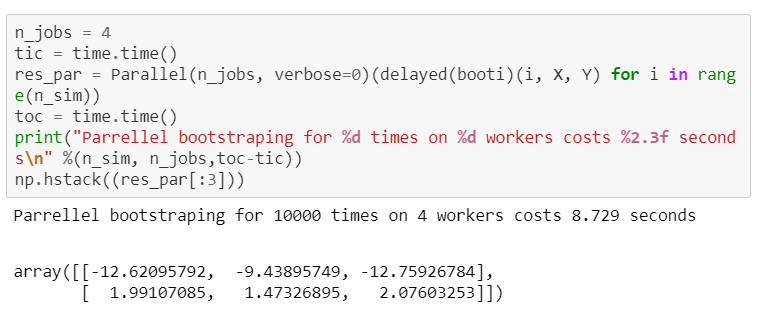
\includegraphics[width=0.85\linewidth]{figure/screenshot029}
	\end{figure}
	
\end{itemize}
\end{frame}

\begin{frame}
\frametitle{`overhead' and memory mapped file}
	\begin{itemize}
		\item Not exactly 4 times faster because of \textcolor{blue}{`overhead'} (extra time on copying data for each worker, communication etc.)
		\item \textcolor{blue}{Memory mapped file}:  a chunk of memory whose bytes are accessible by more than one process 
		\begin{itemize}
			\item Save space: avoid copying dataset repeatedly
			\item Save time : reduce "overhead"
		\end{itemize}
			\item \texttt{dump} and \texttt{load}
		\begin{figure}
			\centering
			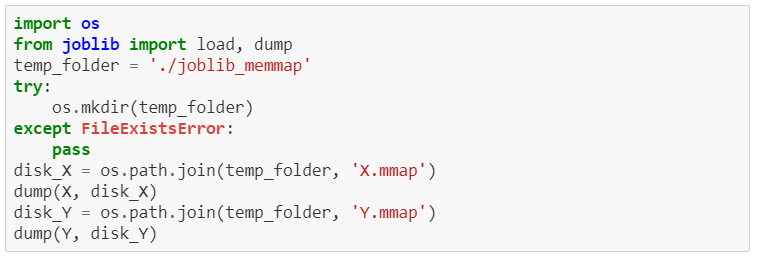
\includegraphics[width=1\linewidth]{figure/screenshot030}
		\end{figure}
	\end{itemize}

\end{frame}

\begin{frame}
\frametitle{Effect of memory mapped file}
\begin{itemize}
	\item With \texttt{memmap} file:
	\begin{figure}
		\centering
		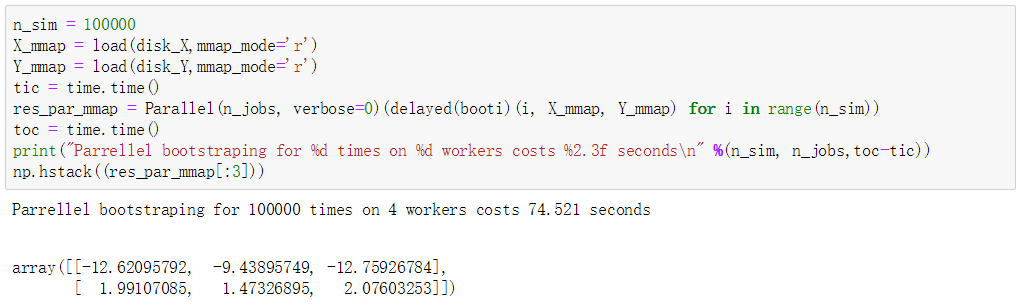
\includegraphics[width=1\linewidth]{figure/screenshot037}
	\end{figure}
	
	\item Without  \texttt{memmap} file:
	\begin{figure}
		\centering
		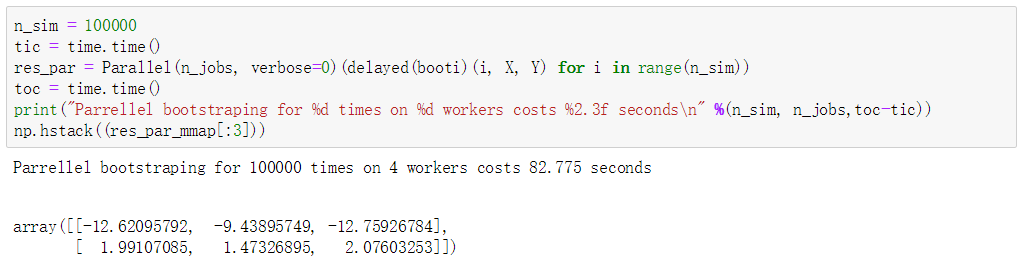
\includegraphics[width=1\linewidth]{figure/screenshot038}
	\end{figure}
\end{itemize}
\end{frame}
\begin{frame}
\centering
\LARGE \textcolor{blue}{\textbf{Web scrapping using \texttt{Beautiful Soup}}}
\end{frame}

\begin{frame}
\frametitle{Before you start}
\begin{itemize}
	\item \textbf{Do you really need scrapping?} check if the website has public API or dataset available.
	\item Before scrapping: check the \textcolor{blue}{website policy}
	\item \textcolor{blue}{Download} webpages first to avoid requesting repeatedly
	\begin{figure}
		\centering
		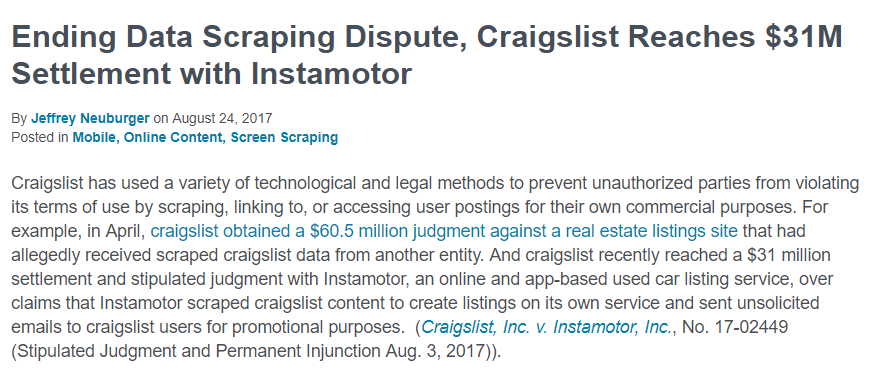
\includegraphics[width=1\linewidth]{figure/screenshot039}
	\end{figure}
	
\end{itemize}
\end{frame}

\begin{frame}
\frametitle{Example: get artist information from national gallery}
\begin{itemize}
	\item National Gallery artist directory: https://web.archive.org/web/20121007172955/https://www.nga.gov/
	collection/anZ1.htm
	\item Save first by \textcolor{blue}{\texttt{requests.get}}
	\begin{figure}
		\centering
		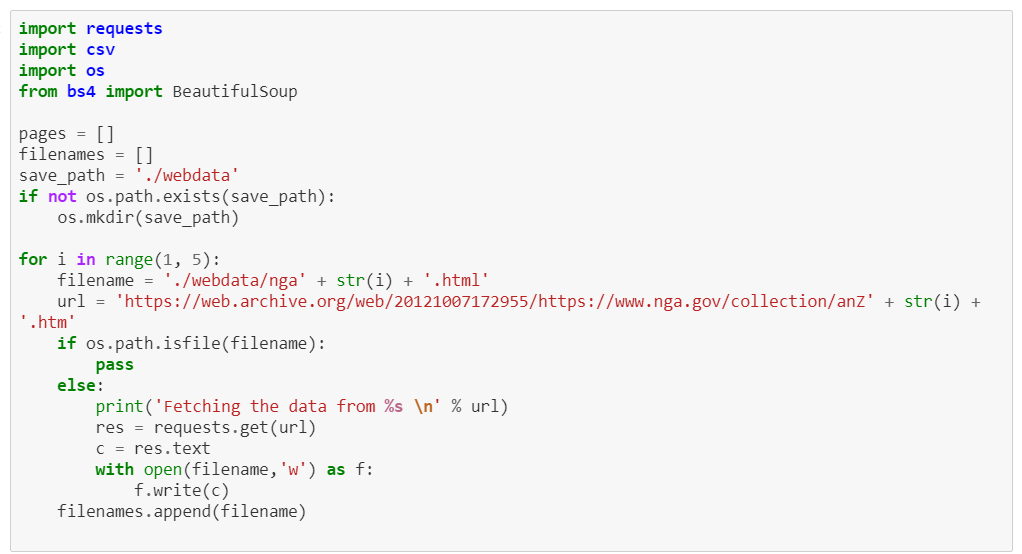
\includegraphics[width=1\linewidth]{figure/screenshot031}
	\end{figure}
\end{itemize}
\end{frame}

\begin{frame}
\frametitle{Know your html}
\begin{itemize}
	\item Inspect the page and locate the field you want to scrape
	\begin{figure}
		\centering
		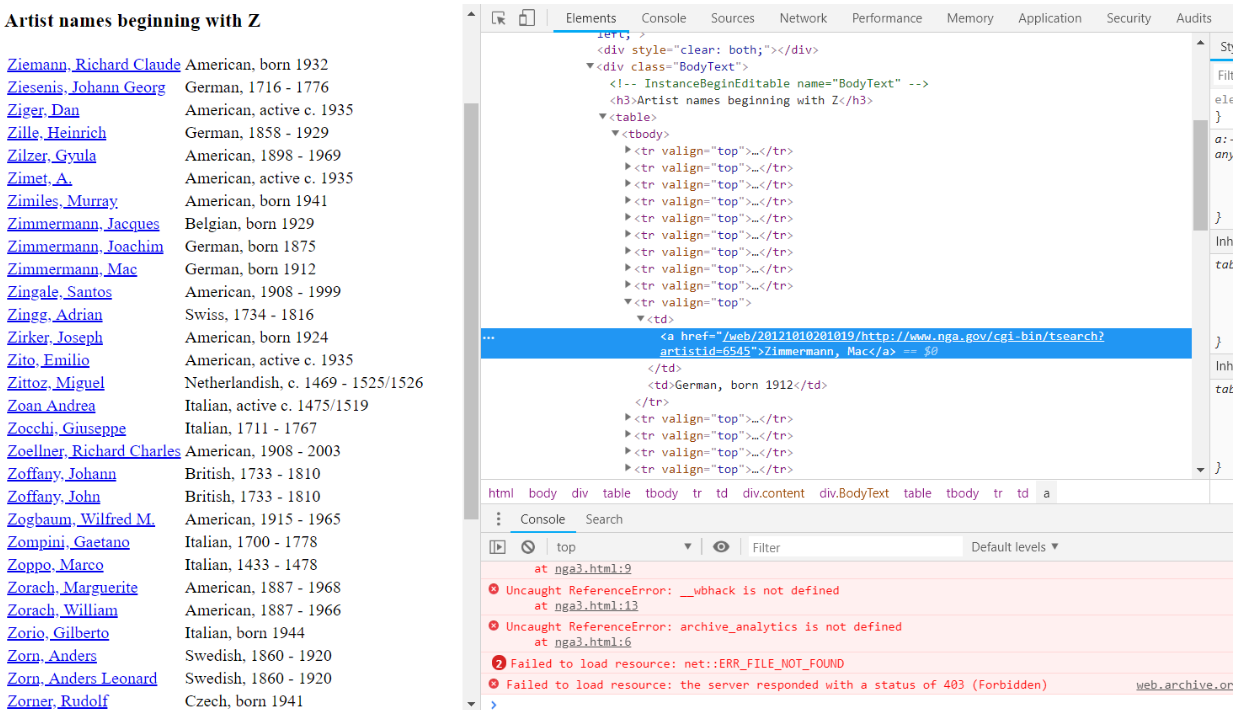
\includegraphics[width=1\linewidth]{figure/screenshot032}
	\end{figure}
\end{itemize}
\end{frame}

\begin{frame}
\frametitle{Search your html}
\begin{enumerate}
	\item Target texts are wrapped in \textcolor{blue}{\texttt{<div class="BodyText">}} and always start with \textcolor{blue}{\texttt{a}}.
	\item Use \texttt{soup.find} to fetch the data
	\begin{figure}
		\centering
		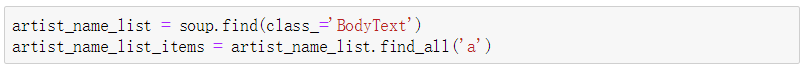
\includegraphics[width=1\linewidth]{figure/screenshot033}
	\end{figure}
	\item Obtain the name by \texttt{artist\_name\textcolor{blue}{.contents}}
	\item Obtain the link by \texttt{artist\_name\textcolor{blue}{.get('href')}}
	\item Exclude the unrelated text
	\begin{figure}
		\centering
		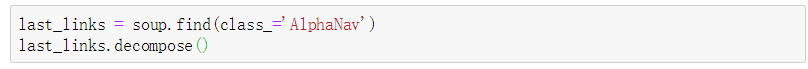
\includegraphics[width=1\linewidth]{figure/screenshot034}
	\end{figure}
	\item Save the data to \texttt{.csv} file
\end{enumerate}
\end{frame}

\begin{frame}
\frametitle{Full code}
\begin{figure}
	\centering
	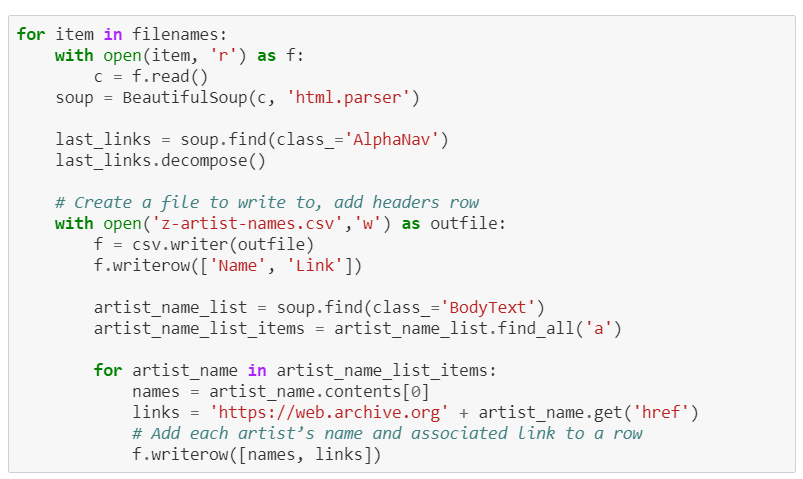
\includegraphics[width=1\linewidth]{figure/screenshot035}
\end{figure}
\end{frame}

\begin{frame}
\frametitle{Result}
\begin{figure}
	\centering
	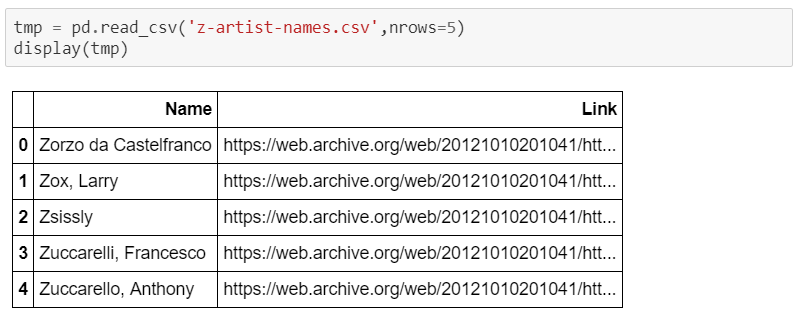
\includegraphics[width=1\linewidth]{figure/screenshot036}
\end{figure}
\end{frame}

\begin{frame}
\frametitle{Other cool stuffs}
\begin{itemize}
	\item \textcolor{blue}{\texttt{mmap}}: memory-mapping file
	\vspace{2mm}
	\item \textcolor{blue}{\texttt{Spark}} and \textcolor{blue}{\texttt{PySpark}}: use "Apache Arrow" to enjoy the familiar pandas syntax and the speed of Spark
	\vspace{2mm}
	\item \textcolor{blue}{\texttt{datatable}}: Python version of \texttt{data.table} in R. (\textbf{No windows versoin available so far})
	\vspace{2mm}
	\item Large data processing benchmark comparison:
	https://h2oai.github.io/db-benchmark/
\end{itemize}
\end{frame}

\begin{frame}
\frametitle{Homework1 on Compass}
\begin{itemize}
	\item Due on \textbf{Feb.11,11:59pm}
	\item Scrape data from https://www.isws.illinois.edu/statecli/cuweather/
	\item \textcolor{red}{\textbf{The format of the pages changes over time!}}
	\item Hint:
	\begin{figure}
		\centering
		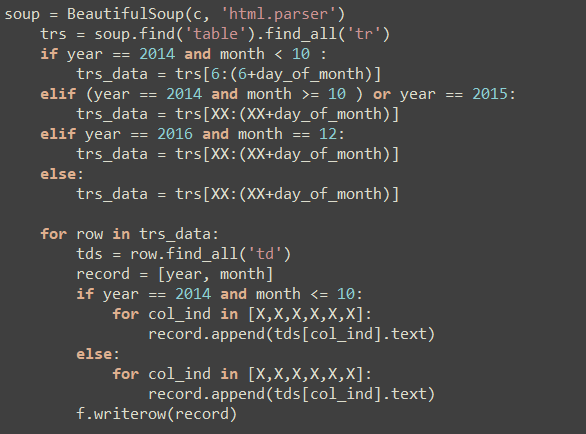
\includegraphics[width=0.7\linewidth]{figure/screenshot040}
	\end{figure}
	
\end{itemize}

\end{frame}

\begin{frame}
\frametitle{Get ready for Deep Learning}
\begin{itemize}
	\item Packages required: \texttt{tensorflow} (Python 3.4, 3.5, 3.6), \texttt{keras, skopt}
	\item Check installation guide: \texttt{pip, conda}
	\begin{figure}
		\centering
		\includegraphics[width=0.7\linewidth]{godeeper}
	\end{figure}
	
	
\end{itemize}
\end{frame}

\begin{frame}
\frametitle{Acknowledgment and references}
\begin{itemize}
	\item These tutorial is inspired by the following posts:
	\vspace{2mm}
	\begin{itemize}
		\item https://plot.ly/ipython-notebooks/big-data-analytics-with-pandas-and-sqlite/
		\item https://www.dataquest.io/blog/pandas-big-data/.
		\item https://www.digitalocean.com/community/tutorials/how-to-scrape-web-pages-with-beautiful-soup-and-python-3
	\end{itemize}
	\vspace{2mm}
	\item  Special thanks to James Balamuta for his advice
\end{itemize}

\end{frame}



\end{document}